% The quotient of the plane by a line W: the classes are the lines parallel to W; a complement C meets each once.
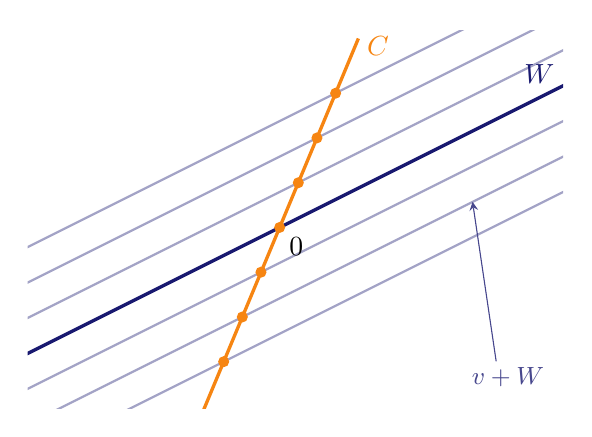
\begin{tikzpicture}[>=stealth]
\begin{scope}
\clip (-3.2,-2.3) rectangle (3.6,2.5);
\draw[MidnightBlue!40,thick] (-4.000,-0.650) -- (4.000,3.350);
\draw[MidnightBlue!40,thick] (-4.000,-1.100) -- (4.000,2.900);
\draw[MidnightBlue!40,thick] (-4.000,-1.550) -- (4.000,2.450);
\draw[MidnightBlue!40,thick] (-4.000,-2.450) -- (4.000,1.550);
\draw[MidnightBlue!40,thick] (-4.000,-2.900) -- (4.000,1.100);
\draw[MidnightBlue!40,thick] (-4.000,-3.350) -- (4.000,0.650);
\draw[MidnightBlue,very thick] (-4,-2) -- (4,2);
\draw[BurntOrange,very thick] (-1.0,-2.4) -- (1.0,2.4);
\fill[BurntOrange] (0.711,1.705) circle (2pt);
\fill[BurntOrange] (0.474,1.137) circle (2pt);
\fill[BurntOrange] (0.237,0.568) circle (2pt);
\fill[BurntOrange] (-0.000,-0.000) circle (2pt);
\fill[BurntOrange] (-0.237,-0.568) circle (2pt);
\fill[BurntOrange] (-0.474,-1.137) circle (2pt);
\fill[BurntOrange] (-0.711,-1.705) circle (2pt);
\end{scope}
\node[MidnightBlue] at (3.3,1.95) {$W$};
\node[BurntOrange] at (1.25,2.3) {$C$};
\node[below right] at (0,0) {$0$};
\node[MidnightBlue!80,font=\small] at (2.9,-1.9) {$v+W$};
\draw[->,MidnightBlue!80] (2.75,-1.7) -- (2.45,0.325);
\end{tikzpicture}
